\section{Постановка задачи}

\begin{frame}[t]{Исследование пещер}


    \begin{columns}[T,onlytextwidth]
        \begin{column}{0.62\textwidth}
            \small
                \textbf{Назначение} --- геологоразведка, изучение подземных экосистем
            \begin{exampleblock}{Непроходимые места для человека}
                \begin{itemize}
                    \item Узкие галереи, огромные пропасти, обвалы, сифоны
                    \item Скопление угарного газа
                    \item Потеря ориентации в пространстве
                \end{itemize}
            \end{exampleblock}
            \vspace{-0.2cm}
            \begin{alertblock}{Заинтересованные стороны}
                \begin{enumerate}
                    \item \textit{Ученые} --- Горный институт Уральского отделения РАН, Университет Минас-Жерайса, Фонд Бруно Кесслера
                    \item \textit{Космические агентства} --- ESTEC (DAEDALUS), Роскосмос (FEDOR), NASA (CADRE)
                    \item \textit{Военные} --- Darpa Subterranean Challenge
                \end{enumerate}
            \end{alertblock}
        \end{column}
        \begin{column}{0.37\textwidth}
            \begin{figure}[H]
                \begin{subfigure}{0.49\textwidth}
                    \centering\includegraphics[height=2cm,width=1\textwidth,keepaspectratio]{../images/slides/rip.jpg}
                    \caption*{Могила}
                \end{subfigure}
                \begin{subfigure}{0.49\textwidth}
                    \centering\includegraphics[height=2cm,width=1\textwidth,keepaspectratio]{../images/surface_types/siphon.png}
                    \caption*{Сифоны}
                \end{subfigure}
            
                \begin{subfigure}{0.49\textwidth}
                    \centering\includegraphics[height=2cm,width=1\textwidth,keepaspectratio]{../images/slides/daedalus.jpg}
                    \caption*{DAEDALUS для исследования пещер на луне}
                \end{subfigure}
                \begin{subfigure}{0.49\textwidth}
                    \centering\includegraphics[height=2cm,width=1\textwidth,keepaspectratio]{../images/open_cave.jpg}
                    \caption*{DARPA Subterranean Challenge}
                \end{subfigure}
            \end{figure}
        \end{column}
    \end{columns}
\end{frame}

\note{
\small \setlength{\parindent}{20pt}    
Одним из способов нахождения новых минералов или форм жизни является исследование пещер спелеологами. Но данное мероприятие очень опасно, так как в пещерах можно встретить обвалы, сифоны *тык*, можно потеряться. Также возможно задохнуться от угарного газа.

Поэтому разные организации во всем мире пытаются начать применять робот при исследовании пещер. Это как и ученые из России, к примеру Горный институт Уральского отделения РАН, с которым Иннополис подписал бумагу о совместных исследования, а также к примеру университет Минас-Жрелайса в Бразилии или фонд Бруно Кесслера в Италии.

Пещеры находятся не только на Земле, поэтому космические агентства всего мира также активно развивают данную область. К примеру *тык* Европейское агентво собирается скоро отправить робота Дедала для исследования пещер на луне.

Нахождение новых минералов и форм жизни, а также способы автономной навигации в таких сложных местах, может помочь в развитии военной промышленности. Это понимает Американское Военное агенство --- DARPA, проводя конкурс DARPA Subterranean Challenge *тык*, где роботы в полностью автономном режиме должны исследовать различные виды пещер.}

\begin{frame}[t]{Характеристики пещер}
    \framesubtitle{}
    \vspace{-0.8cm}
    \begin{figure}[H]
        \begin{subfigure}{0.49\textwidth}
            \begin{subfigure}[b]{0.49\textwidth}
                \centering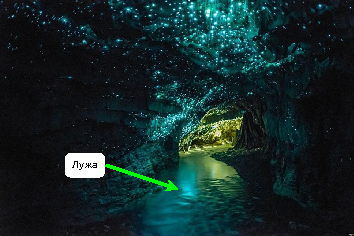
\includegraphics[height=2.5cm,width=1\textwidth,keepaspectratio,page=1]{./tikz_pictures.pdf}
                \caption{Лужа}
            \end{subfigure}
            \hfill
            \begin{subfigure}[b]{0.49\textwidth}
                \centering\includegraphics[height=2.5cm,width=1\textwidth,keepaspectratio]{surface_types/moss.jpg}\\
                \caption{Мох}
            \end{subfigure}

            \begin{subfigure}[b]{0.49\textwidth}
                \centering\includegraphics[height=2.5cm,width=1\textwidth,keepaspectratio]{surface_types/salt.jpg}\\
                \caption{Твердые породы}
            \end{subfigure}
            \begin{subfigure}[b]{0.49\textwidth}
                \centering\includegraphics[height=2.5cm,width=1\textwidth,keepaspectratio]{surface_types/sand.jpg}\\
                \caption{Земля}
            \end{subfigure}
            \caption*{Типы опорных поверхностей}
        \end{subfigure}
        \begin{subfigure}{0.49\textwidth}
            \begin{subfigure}{0.99\textwidth}
                \centering\includegraphics[height=3cm,width=1\textwidth,keepaspectratio]{../images/human_crawling.png}
                \caption*{Габариты пещеры (Свободная узость)}
            \end{subfigure}

            \begin{subfigure}{0.99\textwidth}
                \centering\includegraphics[height=3cm,width=1\textwidth,keepaspectratio]{../images/cave_maps/map3.png}
                \caption*{Протяженность пещер: 1--2 км}
            \end{subfigure}
        \end{subfigure}
    \end{figure}
\end{frame}

\note{\small \setlength{\parindent}{20pt} 
Так как пещеры бывают абсолютно разными, я решил ограничить спектр пещер для которых решалась задача. Слева представлены типы опорных поверхностей, которые могут встречаться в пещерах *тык*. Это земляной грунт, малые водяные препятствия или лужи, твердые породы, а также мох.

Для разработки объекта исследования необходимо понимать также и габариты пещер, а также их протяженность. Изучив различные карты пещер, такие как на рисунке внизу *тык* было решено взять протяженность пещер в диапазоне от 1 до 2ух км.

Основная задача это исследовать пещеры, которые не может исследовать человек физически из-за ограничения размеров. Человеку сложно долго ползать на четвереньках, поэтому я решил так, что робот должен быть как минимум меньше, чем средний мужчина в габаритах *тык*. А именно 600х1000х600 мм. Такой тип препятствий в спелеологии называется свободная узость.
}

\begin{frame}[t]{Некорректные данные с оптических сенсоров}
    \framesubtitle{}
    \begin{figure}[H]
        \begin{subfigure}[t]{0.49\textwidth}
            \centering\includegraphics[height=5cm,width=1\textwidth,keepaspectratio]{../images/moh_damping.jpg}
            \caption*{Мох приминается после ходьбы}
        \end{subfigure}
        \begin{subfigure}[t]{0.49\textwidth}
            \centering\includegraphics[height=5cm,width=1\textwidth,keepaspectratio,page=2]{./tikz_pictures.pdf}
            \caption*{Лазер отражается от воды, а камера не различает объекты в мутной воде}
        \end{subfigure}
    \end{figure}
\end{frame}

\note{\small \setlength{\parindent}{20pt}
Для исследования пещер роботу нужна система навигации. Классические системы навигации основаны на оптических сенсорах.

К сожалению, в пещерах встречаются случаи, когда оптические сенсоры: лидары, камеры, не смогут достоверно построить карту.

К примеру, мох *тык*. Он меняет свой объем при наступании на него и это возможно только измерить во время ходьбы. До или после будут уже другой рельеф. 

Второй пример --- построение опорной поверхности под лужей *тык*. Лидар будет отражаться от поверхности воды и построит гладкую поверхность, а камера не будет работать в мутной воде, как и зеленый лидар.

С использованием же разработанных методов, данная задача решаема, что и будет показано далее.
}

\begin{frame}[t]{Цель работы}
    \framesubtitle{}
    Разработать \textbf{метод построения карты местности} с определением \underline{геометрических} и \underline{физико-механических} свойств \textit{опорной поверхности} роботом с шагающими движителями снабженными \underline{тактильными датчиками}, \textit{без использования оптических сенсоров}.
    \begin{figure}[H]
        \begin{subfigure}{0.49\textwidth}
            \centering\includegraphics[height=4cm,width=1\textwidth,keepaspectratio]{../images/slides/geom_prop.png}
            \caption*{Определение геометрических свойств}
        \end{subfigure}
        \begin{subfigure}{0.49\textwidth}
            \centering\includegraphics[height=4cm,width=1\textwidth,keepaspectratio]{s_shape_leg/view.jpg}
            \caption*{Определение физических свойств}
        \end{subfigure}
    \end{figure}
\end{frame}

\note{\small \setlength{\parindent}{20pt}
Целью работы являлось разработать метод построения карты местности роботом с шагающими движителями, у которого на стопах установлены датчики силы. Задача должна решаться без использования оптических сенсоров.

Я разбил понятие построения карты на две задачи: определение геометрических свойств *тык* и физико - механических *тык*.

}

\begin{frame}[t]{"1, 2" Построение рельефа местности}
    \framesubtitle{}
    \begin{columns}[T,onlytextwidth]
        \begin{column}{0.49\textwidth}
            \textbf{Геометрические свойства:}\\
            \textit{Входные данные}: следовая дорожка, представленная в виде облака точек.

            \textit{Выходные данные}: полигональная сетка и плотное облако точек.

            \textit{Допустимая точность}: 0.1 м
            \begin{figure}[H]
                \begin{subfigure}[t]{0.49\textwidth}
                    \centering\includegraphics[height=2cm,width=1\textwidth,keepaspectratio]{../images/slides/surface_research.png}
                    \caption*{Исследуемая поверхность}
                \end{subfigure}
                \begin{subfigure}[t]{0.49\textwidth}
                    \centering\includegraphics[height=2cm,width=1\textwidth,keepaspectratio]{../images/slides/result_research.png}
                    \caption*{Следовая дорожка и полигональная сетка}
                \end{subfigure}
            \end{figure}
        \end{column}
        \begin{column}{0.49\textwidth}
            \textbf{Физико-механические свойства:}\\
            \textit{Входные данные}: данные с внутренних датчиков робота.

            \textit{Выходные данные}: процентное соотношение упругих, твердых и пластичных свойств пройденной поверхности.

            \textit{Допустимая ошибка}: 20\% 

            \vspace{-0.35cm}
            \begin{figure}[H]
                \begin{subfigure}[t]{0.49\textwidth}
                    \centering\includegraphics[height=2.5cm,width=1\textwidth,keepaspectratio]{../images/slides/avg_lin_vel_rev_min.png}
                    \caption*{Данные для обучения}
                \end{subfigure}
                \begin{subfigure}[t]{0.49\textwidth}
                    \centering\includegraphics[height=2.5cm,width=1\textwidth,keepaspectratio]{../images/slides/data.png}
                    \caption*{Пример поверхности}
                \end{subfigure}
            \end{figure}
        \end{column}
    \end{columns}
\end{frame}

\note{\small \setlength{\parindent}{20pt}

Задачи 1 и 2 - определение геометрических и физико-механических свойств опорной поверхности. Хочу отметить, что задачи пронумерованы в порядке значимости, но не в порядке выполнения.

Рассматривая геометрические свойства, то входными данными я считаю следовую дорожку, которая представлена в виде облака точек, относительно абсолютных систем координат.

Результатом примененного метода решения должны получиться полигональная сетка пройденной поверхности, а также плотное облако точек. Эти представления являются типичными способами представления для работы с навигацией. *тык*. Синие точки --- следовая дорожка, зеленым цветом --- полигональная сетка

Целью же определения физико-механических свойств является определение какие свойства у пройденной поверхности превалируют: твердые, упругие или пластичные. Решение задачи основано на обучении модели машинного обучения на данных с внутренних датчиков робота *тык*. К примеру одним из примером данных является частота вращения ног.

Более точные формулировки задач с алгоритмом и принятыми предположениями будут далее.}

\begin{frame}[t]{Объект исследования}
    \framesubtitle{}
    \begin{columns}[T,onlytextwidth]
        \begin{column}{0.49\textwidth}
            \textbf{Класс многоногих шагающих роботов} с \\
            а) \underline{Цельным} или \underline{сочленённым} \textit{корпусом}\\
            б) \underline{Цикловыми} \textit{движителями} с \underline{одной степенью свободы}, управляемые зависимо или независимо друг от друга.

            \textit{Требования}:
            \begin{itemize}
                \item Компактные размеры (меньше чем $1000\times600\times600$ мм)
                \item Залезать на препятствия высотой не меньше, чем $\frac{3}{4}$ длины корпуса
                \item Преодолевать представленные
                      опорные поверхности
            \end{itemize}
        \end{column}
        \begin{column}{0.49\textwidth}
            \begin{figure}[H]
                \hfill
                \begin{subfigure}{0.99\textwidth}
                    \centering\includegraphics[height=2.5cm,width=1\textwidth,keepaspectratio]{from_master/whegs2.jpg}
                    \caption*{WHegs}
                \end{subfigure}

                \hfill
                \begin{subfigure}[t]{0.49\textwidth}
                    \centering\includegraphics[height=2.5cm,width=1\textwidth,keepaspectratio]{from_master/rhex.jpg}
                    \caption*{Boston Dynamics RHex}
                \end{subfigure}
                \begin{subfigure}[t]{0.49\textwidth}
                    \centering\includegraphics[height=2.5cm,width=1\textwidth,keepaspectratio]{from_master/gakken.jpg}
                    \caption*{Gakken Centipede}
                \end{subfigure}
            \end{figure}
        \end{column}
    \end{columns}
\end{frame}

\note{\small \setlength{\parindent}{20pt}
Рассмотрев различные варианты роботов, было решено выбрать класс многоногих шагающих роботов с цельным или сочлененным корпусом и цикловыми движителями с одной степенью свободы, управляемые зависимо или независимо друг от друга.

Такой класс был выбран так как его представители показывают высокие показания профильной проходимости, что видно в видео справа *тык*. На рисунках представлены разные представители --- вхегс, рхекс, сентипеде *тык*.

У вхегс 6 ног и 1 активное сочленение, у Рхекса также 6 ног, но один корпус. У обоих ноги управляются независимо. У Гаккен сентипеде же 32 ноги, нет сочленений, а движение одной ноги зависит от положения другой.

Данных класс роботов может соответствовать поставленным требованиям.Нужно, чтобы разработанный роботом меньше габаритов пещеры, мог залезать на препятствия высотой не меньше, чем ¾ длины корпуса, а также мог физически преодолевать препятствия, которые были заявлены как те, которые можно встретить в пещере.
}

\begin{frame}[t]{"3" Оптимизация кинематической схемы}
    \framesubtitle{}
    \begin{columns}[T,onlytextwidth]
        \begin{column}{0.45\textwidth}
            Решить задачу оптимизации $F=f(x) \rightarrow max$, где

            $f(x)$ --- критерии: пройденная дистанция, длина корпуса\\
            $(x)$ --- параметр: \textbf{количество ног}
            \medskip

            \textit{Количество ног имеет прямую зависимость с длиной корпуса робота.}
        \end{column}
        \begin{column}{0.54\textwidth}
            \vspace{-0.5cm}
            \begin{figure}[H]
                \begin{subfigure}{0.99\textwidth}
                    \centering\includegraphics[height=1.8cm,width=1\textwidth,keepaspectratio]{f1.png}
                    \caption*{Кол-во ног $\uparrow$, детализация поверхности $\uparrow$}
                \end{subfigure}

                \begin{subfigure}{0.99\textwidth}
                    \centering\includegraphics[height=1.8cm,width=1\textwidth,keepaspectratio]{f2.png}
                    \caption*{Длина робота $\uparrow$, курсовая проходимость $\downarrow$}
                \end{subfigure}

                \begin{subfigure}{0.99\textwidth}
                    \centering\includegraphics[height=1.8cm,width=1\textwidth,keepaspectratio]{f3_new.png}
                    \caption*{Длина робота $\uparrow$, профильная проходимость $\uparrow$}
                \end{subfigure}
            \end{figure}
        \end{column}
    \end{columns}
\end{frame}

\note{\small \setlength{\parindent}{20pt}

У различных представителей этого класса, разное количество ног. Более того, количество ног также влияет и на построение карты, так как если у робота ног больше, то карта будет более детализированной *тык*, а следовательно - точнее. 

Но с другой стороны, пещеры имеют много изгибов и при большой длине робот может застрять *тык*. То есть чем длинее робот, тем хуже курсовая проходимость. 

Более длинный робот может преодолевать больше препятствий, как это показано на рисунке *тык*. Он не провалится в яму, а из-за своей длины сможет ее пересечь.

Следовательно у нас возникает мультикритериальная задача оптимизации, где критерием является пройденная дистанция и длина корпуса. И задача - определить оптимальное количество ног.
}

\begin{frame}[t]{"4" Верификация преобразователя силы}
    \framesubtitle{}
    \begin{columns}[T,onlytextwidth]
        \begin{column}{0.59\textwidth}
            \underline{Измерить характеристики} материала для случаев, когда \textbf{площадь приложения силы меньше}, чем \textbf{площадь активной части} сенсора.

            \textit{Входные данные}: показания разработанного датчика и значение реально приложенной нагрузки

            \textit{Выходные данные}: разница между нормализованным значением с датчика и реальной нагрузкой

            \textit{Допустимая ошибка}: 10\% 
        \end{column}
        \begin{column}{0.39\textwidth}
            \vspace{-0.6cm}
            \begin{figure}[H]
                \begin{subfigure}{0.9\textwidth}
                    \centering\includegraphics[height=1.5cm,width=1\textwidth,keepaspectratio]{velostat_sensor.jpg}
                    \caption*{Материал Velostat}
                \end{subfigure}

                \begin{subfigure}{0.9\textwidth}
                    \centering\includegraphics[height=2cm,width=1\textwidth,keepaspectratio]{simplest_sensor.jpg}
                    \centering\includegraphics[height=2cm,width=1\textwidth,keepaspectratio]{slides/v_sensor_desig.png}
                    \caption*{Преобразователь силы}
                \end{subfigure}
            \end{figure}
        \end{column}
    \end{columns}
\end{frame}

\note{\small \setlength{\parindent}{20pt}

В первичной постановке задачи о построении карты, как для определения геометрических, так и физико-механических свойств, говорилось о том, что на роботе установлены датчики силы. После обзора различных решений, было решено разработать свой пьезорезистивный преобразователь силы на основе Velostat *тык*. Данный материал был выбран из-за его отличного соотношения цена/качество. Так как на робота нужно установить много датчиков на каждую ногу, это является важным фактором.

При изучения данного материала я заметил, что когда площадь приложения силы меньше, чем площадь активной части сенсора, то при одинаковом давлении, показания будут разными. А это будет сильно влиять на работу алгоритмов. Примером является маленький камушек, на который робот наехал при ходьбе.

Поэтому было решено измерить характеристики преобразователя для таких случаев.
}

\begin{frame}[t]{Основные научные задачи исследования}
    \framesubtitle{}
    \begin{enumerate}
        \item  Разработка метода \textbf{построения карты местности и определения геометрических свойств поверхности} с помощью тактильного очувствления.
        \item Реализация алгоритма, позволяющего \textbf{определять физические свойства} опорной поверхности.
        \item Разработка метода \textbf{оптимизации конструкции многоногих шагающих роботов} с цикловыми движителями с одной степенью свободы критериям проходимости, покрытия опорной поверхности и её детализации, длины пройденного пути.
        \item Создание методики \textbf{исследования датчика силы}, когда площадь контакта нажатия на сенсор меньше чувствительной области самого сенсора.
    \end{enumerate}
\end{frame}

\note{\small \setlength{\parindent}{20pt}

Итого получаются следующие научные задачи. Это разработка двух методов --- определение геометрических свойств и оптимизация кинематической схемы, методики по исследованию датчика силы, а также алгоритма определения физико-механических свойств опорной поверхности.
}


\begin{frame}{Положения, выносимые на защиту}
    \begin{enumerate}
        \vspace{-0.3cm}
        \small
        \item \textbf{Метод построения карты местности}, состоящий в определении геометрической формы поверхности с помощью тактильного очувствления, который позволяет решать задачу определения плана и профиля поверхности в условиях отсутствия видимости и при движении по поверхности, находящейся под водой.
        \item \textbf{Метод определения физико-механических свойств опорной поверхности} на основе \textbf{тактильного очувствления}, позволяющий различать материалы с \textit{упругими, жёсткими, пластичными свойствами}.
        \item \textbf{Критерий оптимизации} кинематической схемы многоногих шагающих роботов с цикловыми одностепенными движителями, включающий в себя показатели проходимости, покрытия опорной поверхности и её детализации. Определение на его основе габаритов и количества движителей шагающего робота.
        \item \textbf{Зависимость} \textit{погрешности} датчика силы на основе полимерного материла от \textit{площади пятна контакта} относительно размеров датчика, применяемого для тактильного очувствления мобильного робота. \textbf{Методика} роботизированного исследования датчика силы.
    \end{enumerate}
\end{frame}

\note{\small \setlength{\parindent}{20pt}

На защиту выносятся 2 метода, зависимость и критерий оптимизации кинематической схемы}

\section{Обзор существующих решений}

\begin{frame}[t]{Структура}
    \framesubtitle{}
    \begin{figure}[H]
        \centering\includegraphics[height=6.5cm,width=1\textwidth,keepaspectratio]{main_diag_hor_new.png}
    \end{figure}
\end{frame}

\note{\small \setlength{\parindent}{20pt}

Робот --- сложная система с множеством подсистем и большую часть подсистем я сам лично не делал. На слайде *тык* представлена структура проекта, где оранжевым цветом представлено то, что было разработано мной и где есть научная новизна, а синим - стандартные решения, которые были интегрированы с минимальными наработками.

Так как у целью было построение карты, то робот управлялся в ручном режиме, задача управления была решена максимально тривиально.

Если кратко, то из датчиков на роботе были установлены IMU, энкодеры и датчики силы. Задача локализации решается с помощью системы радио маяков или Aruco маркеров в лаборатории, а из системы технического зрения --- камера, которая также дает и облако точек.
}

\begin{frame}[t]{Обзор источников}
    \framesubtitle{}
    \begin{itemize}
        \item \textbf{Задача оптимизации конструкции}: Б. Петриашвили (СССР), Stefano Nolfi (Италия), Dario Sanch-Pradel (Италия), S. Feng (США) и др.
        \item \textbf{Шагающие цикловые роботы}: Е. С. Брискин (Россия), Ю. Д. Андриантов (СССР), Edward Z. Moore (Канада), Wei-Hsi Chen (Китай) и др.
        \item \textbf{Верификация Velostat}:  Igor Vehec (Словакия),  Robert Schroer (США) и др.
        \item \textbf{Определение геометрических свойств поверхности}: Tobias Ebert (Германия), Subodh Kumar (США), И. Рядчиков (Россия), Shan Luo (Британия) и др.
        \item \textbf{Определение физико-механических свойств поверхности}: X. Alice Wu (США), Krzysztof Walas (Польша), Hendrik Kolvenbach (Швейцария) и др.
    \end{itemize}
\end{frame}

\note{\small \setlength{\parindent}{20pt}

При разработке своих подсистем я базировался на работах следующих ученых со всего мира.

При решении задачи оптимизации количества ног --- на работы Петриашвили, Стефано Нолфи, Feng и других.

Шагающими цикловыми роботами занимается половина это диссертационного совета, поэтому я хочу выделить Эдварда Мура из канады и Wei Hsi из Китая.

В основном материал Велостат исследовал Игорь Вехец, но также были и другие ученые к примеру Роберт Шроер.

Для определения геометрических свойств поверхности, мне пришлось изучить работы ученых из Германии, США, России и Британии.

Мой алгоритм по определению физико-механических свойств в первую очередь базировался на работе пост дока Алисы Ву Стенфордского университета.
}